\documentclass[ms,electronic,oneside,twosidetoc,letterpaper,chaptercenter,parttop]{byumsphd}
% Author: Chris Monson
%
% This document is in the public domain
%
% Options for this class include the following (* indicates default):
%
%   phd (*) -- produce a dissertation
%   ms -- produce a thesis
%
%   electronic -- default official university option, overrides the following:
%                 - equalmargins
%
%   hardcopy -- overrides the following:
%                 - no equalmargins
%                 - twoside
%
%   letterpaper -- ignored, but helpful for the Makefile that I use
%
%   10pt -- 10 point font size
%   11pt -- 11 point font size
%   12pt (*) -- 12 point font size
%
%   lof -- produce a list of figures in the preamble (off)
%   lot -- produce a list of tables in the preamble (off)
%   lol -- produce a list of listings in the preamble (off)
%
%   layout -- show layout lines on the pages, helps with overfull boxes (off)
%   grid -- show a half-inch grid on every page, helps with printing (off)
%   separator -- print an extra instruction page between preamble and body (off)
%
%   twoside (*) -- two-sided output (margins alternate for odd and even pages,
%     blank pages inserted to ensure that chapters begin on the right side of a
%     bound copy, etc.)
%   oneside -- one-sided output (margins are the same on all pages)
%   equalmargins -- make all margins equal - ugly for binding, but compliant
%
%   twosidetoc - start two-sided margins at the TOC instead of the body.  This
%     is sometimes (oddly) required, but be aware that it will make the page
%     numbering seem screwy, e.g., the first four full sheets of paper will
%     have number i-iv (not shown, though), and the next sheets will each have
%     two numbers, one for each side.  I suspect that most people don't look at
%     the roman numerals anyway, but it is a weird requirement.
%
%   openright (*) -- force new chapters to start on an odd page
%   openany -- don't use this, it's ugly
%
%   prettyheadings -- make the section/chapter headings look nice
%   compliantheadings (*) -- make them look ugly, but compliant with standards
%
%   chaptercenter -- center the chapter headings horizontally
%   chapterleft (*) -- place chapter headings on the left
%
%   partmiddle -- Part headers are centered vertically, no other text on page
%   parttop (*) -- Part headers at top of page, other text expected
%
%   duplexprinter -- Ensures that the two-sided portion starts on the right
%     side when printing.  This is not for use in submission, since the best
%     thing to do there is to print everything out one-sided, then take it down
%     to the copy store to have them do the rest.  It does help to save trees
%     when you are printing out copies just to look at them and fiddle with
%     things.
%
%
% EXAMPLES:
%
% The rest is up to you.  To fiddle with margins, use the \settextwidth and
% \setbindingoffset macros, described below.  I suggest that you
% \settextwidth{6.0in} for better-looking output (otherwise you'll get 3/4-inch
% margins after binding, which is sort of weird).  This will depend on the
% opinions of the various dean/coordinator folks, though, so be sure to ask
% them before embarking on a major formatting task.

% The following command fixes my particular printer, which starts 0.03 inches
% too low, shifting the whole page down by that amount.  This shifts the
% document content up so that it comes out right when printed.
%
% Discovering this sort of behavior is best done by specifying the ``grid''
% option in the class parameters above.  It prints a 1/2 inch grid on every
% page.  You can then use a ruler to determine exactly what the printer is
% doing.
%
% Uncomment to shift content up (accounting for printer problems)
%\setlength{\voffset}{-.03in}

% Here we set things up for invisible hyperlinks in the document.  This makes
% the electronic version clickable without changing the way that the document
% prints.  It's useful, but optional.
%
% NOTE: "driverfallback=ps2pdf" chooses ps2pdf in the case of LaTeX and pdftex
% in the case of pdflatex. If you use my LaTeX makefile (at
% http://latex-makefile.googlecode.com/) then pdftex is the default There are
% many other benefits to using the makefile, too.  This option is not always
% available, so use with care.
\usepackage[
    bookmarks=true,
    bookmarksnumbered=true,
    breaklinks=false,
    raiselinks=true,
    pdfborder={0 0 0},
    colorlinks=false,
    plainpages=false,
    ]{hyperref}

% To fiddle with the margin settings use the below.  DO NOT change stuff
% directly (like setting \textwidth) - it will break subtle things and you'll
% be tearing your hair out.
%
% For example, if you want 1.5in equal margins, or 2in and 1in margins when
% printing, add the following below:
%
%\setbindingoffset{1.0in}
%\settextwidth{5.5in}
%
% When equalmargins is specified in the class options, the margins will be
% equal at 1.5in each: (8.5 - 5.5) / 2.  When equalmargins is not specified,
% the inner margin will be 2.0 and the outer margin will be 1.0: inner = (8.5 -
% 5.5 - 1.0) / 2 + 1.0 (the 1.0 is the binding offset).
%
% The idea is this: you determine how much space the text is going to take up,
% whether for an electronic document (equalmargins) or not.  You don't want the
% layout shifting around between printed and electronic documents.
%
% So, you specify the text width.  Then, if there is a binding offset (when
% binding your thesis, the binding takes up space - usually 0.5 inches), that
% reduces the visual space on the final printed copy.  So, the *effective*
% margins are calculated by reducing the page size by the binding offset, then
% computing the remaining space and dividing by two.  Adding back in the
% binding offset gives the inner margin.  The outer margin is just what's left.
%
% All of this is done using the geometry package, which should be manipulated
% directly at your peril.  It's best just to use the above macros to manipulate
% your margins.
%
% That said, using the geometry macro to set top and bottom margins, or
% anything else vertical, is perfectly safe and encouraged, e.g.,
%
%\geometry{top=2.0in,bottom=2.0in}
%
% Just don't fiddle with horizontal margins this way.  You have been warned.

% This makes hyperlinks point to the tops of figures, not their captions
\usepackage[all]{hypcap}

% These packages allow the bibliography to be sorted alphabetically and allow references to more than one paper to be sorted and compressed (i.e. instead of [5,2,4,6] you get [2,4-6])
\usepackage[numbers,sort&compress]{natbib}

% Because I use these things in more than one place, I created new commands for
% them.  I did not use \providecommand because I absolutely want LaTeX to error
% out if these already exist.
\newcommand{\Title}{Cervical Cancer Detection with Synthetic Data and CNNs}
\newcommand{\Author}{Sean Wade}
\newcommand{\GraduationMonth}{December}
\newcommand{\GraduationYear}{2019}

% Set up the internal PDF information so that it becomes part of the document
% metadata.  The pdfinfo command will display this.
\hypersetup{%
    pdftitle=\Title,%
    pdfauthor=\Author,%
    pdfsubject={PhD Dissertation, BYU CS Department: %
                Degree Granted \GraduationMonth~\GraduationYear, Document Created \today},%
    pdfkeywords={BYU, thesis, dissertation, LaTeX},%
}

% Rewrite the itemize, description, and enumerate environments to have more
% reasonable spacing:
\newcommand{\ItemSep}{\itemsep 0pt}
\let\oldenum=\enumerate
\renewcommand{\enumerate}{\oldenum \ItemSep}
\let\olditem=\itemize
\renewcommand{\itemize}{\olditem \ItemSep}
\let\olddesc=\description
\renewcommand{\description}{\olddesc \ItemSep}

% Important settings for the byumsphd class.
\title{\Title}
\author{\Author}

\committeechair{David~Wingate}
\committeemembera{TODO}
\committeememberb{TODO}

\yearcopyrighted{\GraduationYear}

\documentabstract{%
  Cervical cancer is one of the deadliest cancers amoung women worldwide. There are approxiamtly
  270,000 deaths a year, out of which 85\% occure in developing countries. The goal of this project
  is to help in the development of low cost sensors and new algorithms to detect cervical cancer in
  India. Early diagnosis of this cancer is extreamly effective in treatment.

  Recent advances in neural networks can be applied to the early detection of cervical cancer.
  The primary bottleneck is the lack of labeled data and cost of generating it. This project
  will focus on new ways of generating this data and using it in state of the art computer 
  vision algorithms.
}

\documentkeywords{%
    segmentation, CNN, synthetic data, data augmentation, cervical cancer, mediacl imaging
}

\department{Computer~Science}
\graduatecoordinator{Michael~Jones}
%\collegedean{Thomas~W.~Sederberg}
%\collegedeantitle{Associate~Dean}

% Customize the name of the Table of Contents section.
\renewcommand\contentsname{Table of Contents}

% Remove all widows an orphans.  This is not normally recommended, but in a
% paper dissertation there is no reasonable way around it; you can't exactly
% rewrite already-published content to fix the problem.
\clubpenalty 10000
\widowpenalty 10000

% Allow pages to have extra blank space at the bottom in order to accommodate
% removal of widows and orphans.
\raggedbottom

% Produce nicely formatted paragraphs. There is nothing additional to do.  In
% case you get some problems, surround your text with
% \begin{sloppy} ... \end{sloppy}. If that does not work, try
% \microtypesetup{protrusion=false} ... \microtypesetup{protrusion=true}
\usepackage{microtype}
\usepackage{float}
\usepackage{subcaption} % loads the caption package
\usepackage{graphicx}
\graphicspath{ {images/} }

\usepackage{siunitx}


\begin{document}

% Produce the preamble
\microtypesetup{protrusion=false}
\maketitle
\microtypesetup{protrusion=true}

\chapter{Introduction}

Cervical cancer accounts for 6.6\% of cancer cases in the world. In 2018 alone, there were well
over 570,000 cases. Even worse is the disproportionate way populations are affected. About 85\%
of deaths from cervical cancer came from lot to middle income countries.\cite{15}


Fortunatly the high mortality rate from cervical cancer can be reduced by effective screening and early
treatment.

\section{The pap-smear screening}

The pap-smear screening was developed by Georges Papanicolaou. Using a small brush, a cytological sample is taken from the cervix and smeared onto a thin glass slide. 
To clarify the cells characteristics, the smear is stained using the Papanicolaou method. This emphisizes the different components of the cells with specific colors, making it more clear in a microscope.\cite{herlev2}
Each microscope slide contains up to 300,000 single cells with defferent orientations and overlap\cite{herlev2}. This has made automatic segmentation methods challenging.

\chapter{Datasets}

The datasets used are constructed by cyto-technicians for classification purposes. These technicians use a microsope witha resolution of  \SI{0.201}{\micro\metre} / pixel to grab every cell.

\section{SIPaKMeD}

The SIPaKMeD dataset consists of 996 cluser cell images of Pap smear slides. From these there are
4049 indavidual cells that are segmented. These cells are then labeled in 5 categories: 
(a) Dyskeratotic, (b) Koilocytotic, (c) Metaplastic, (d) Parabasal and (e) Superficial-Intermediate.

\begin{figure}[H]
  \centering
  \subcaptionbox{Dysketarotic}{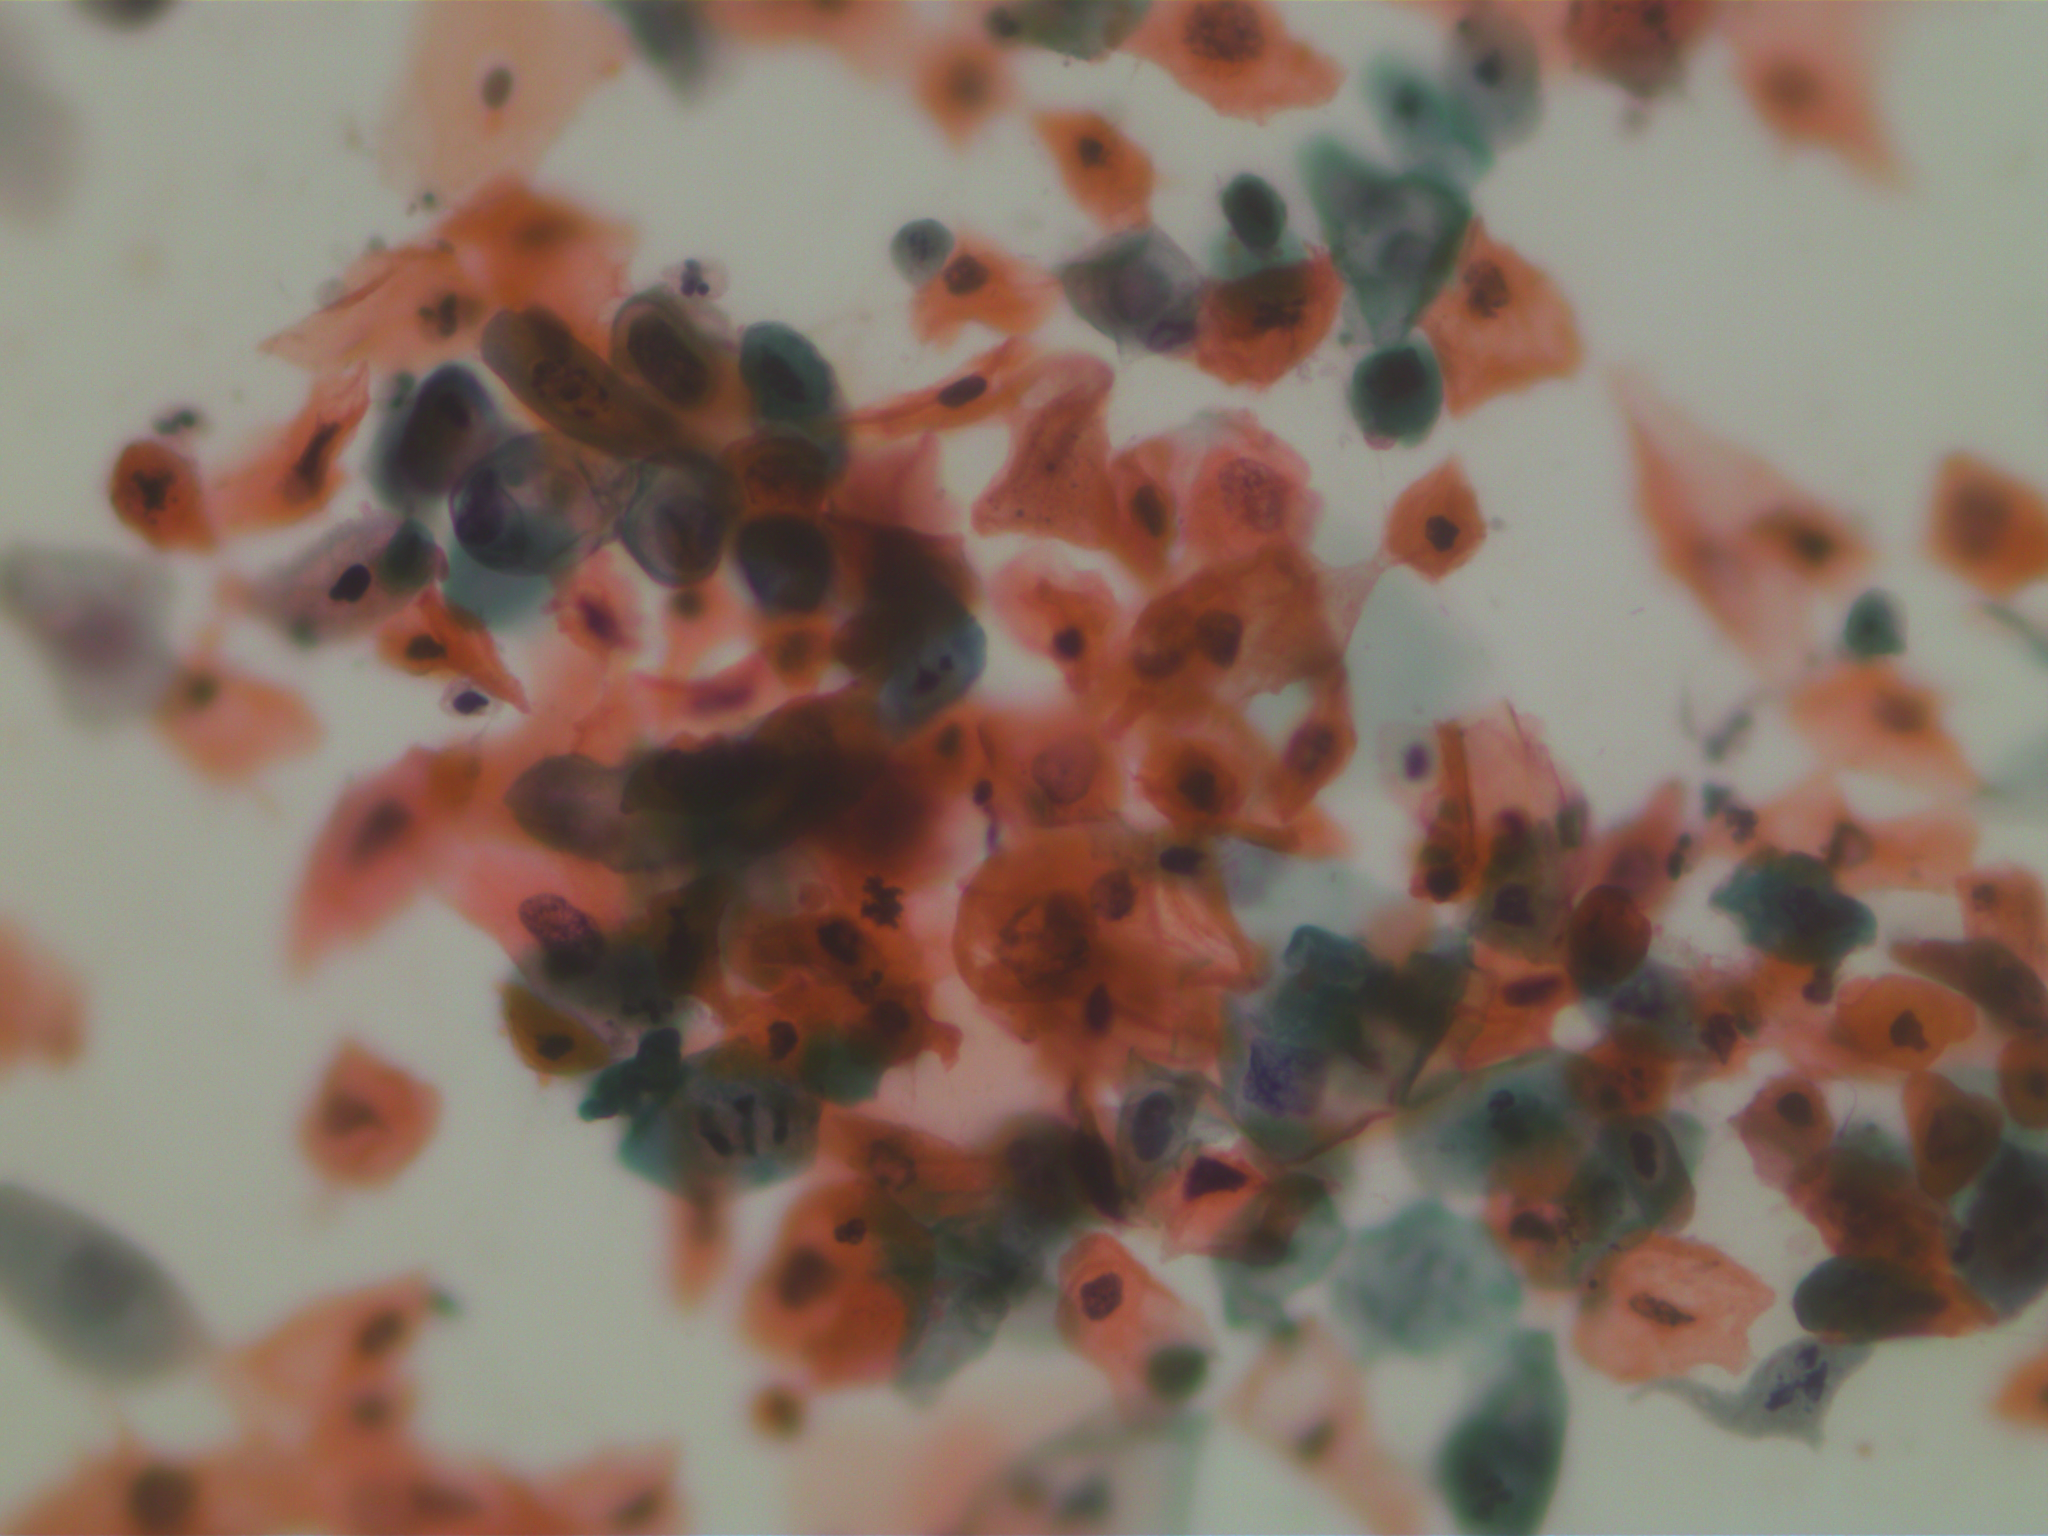
\includegraphics[width=0.30\textwidth]{cells/dysketarotic_059}} \quad
  \subcaptionbox{Koilocytotic}{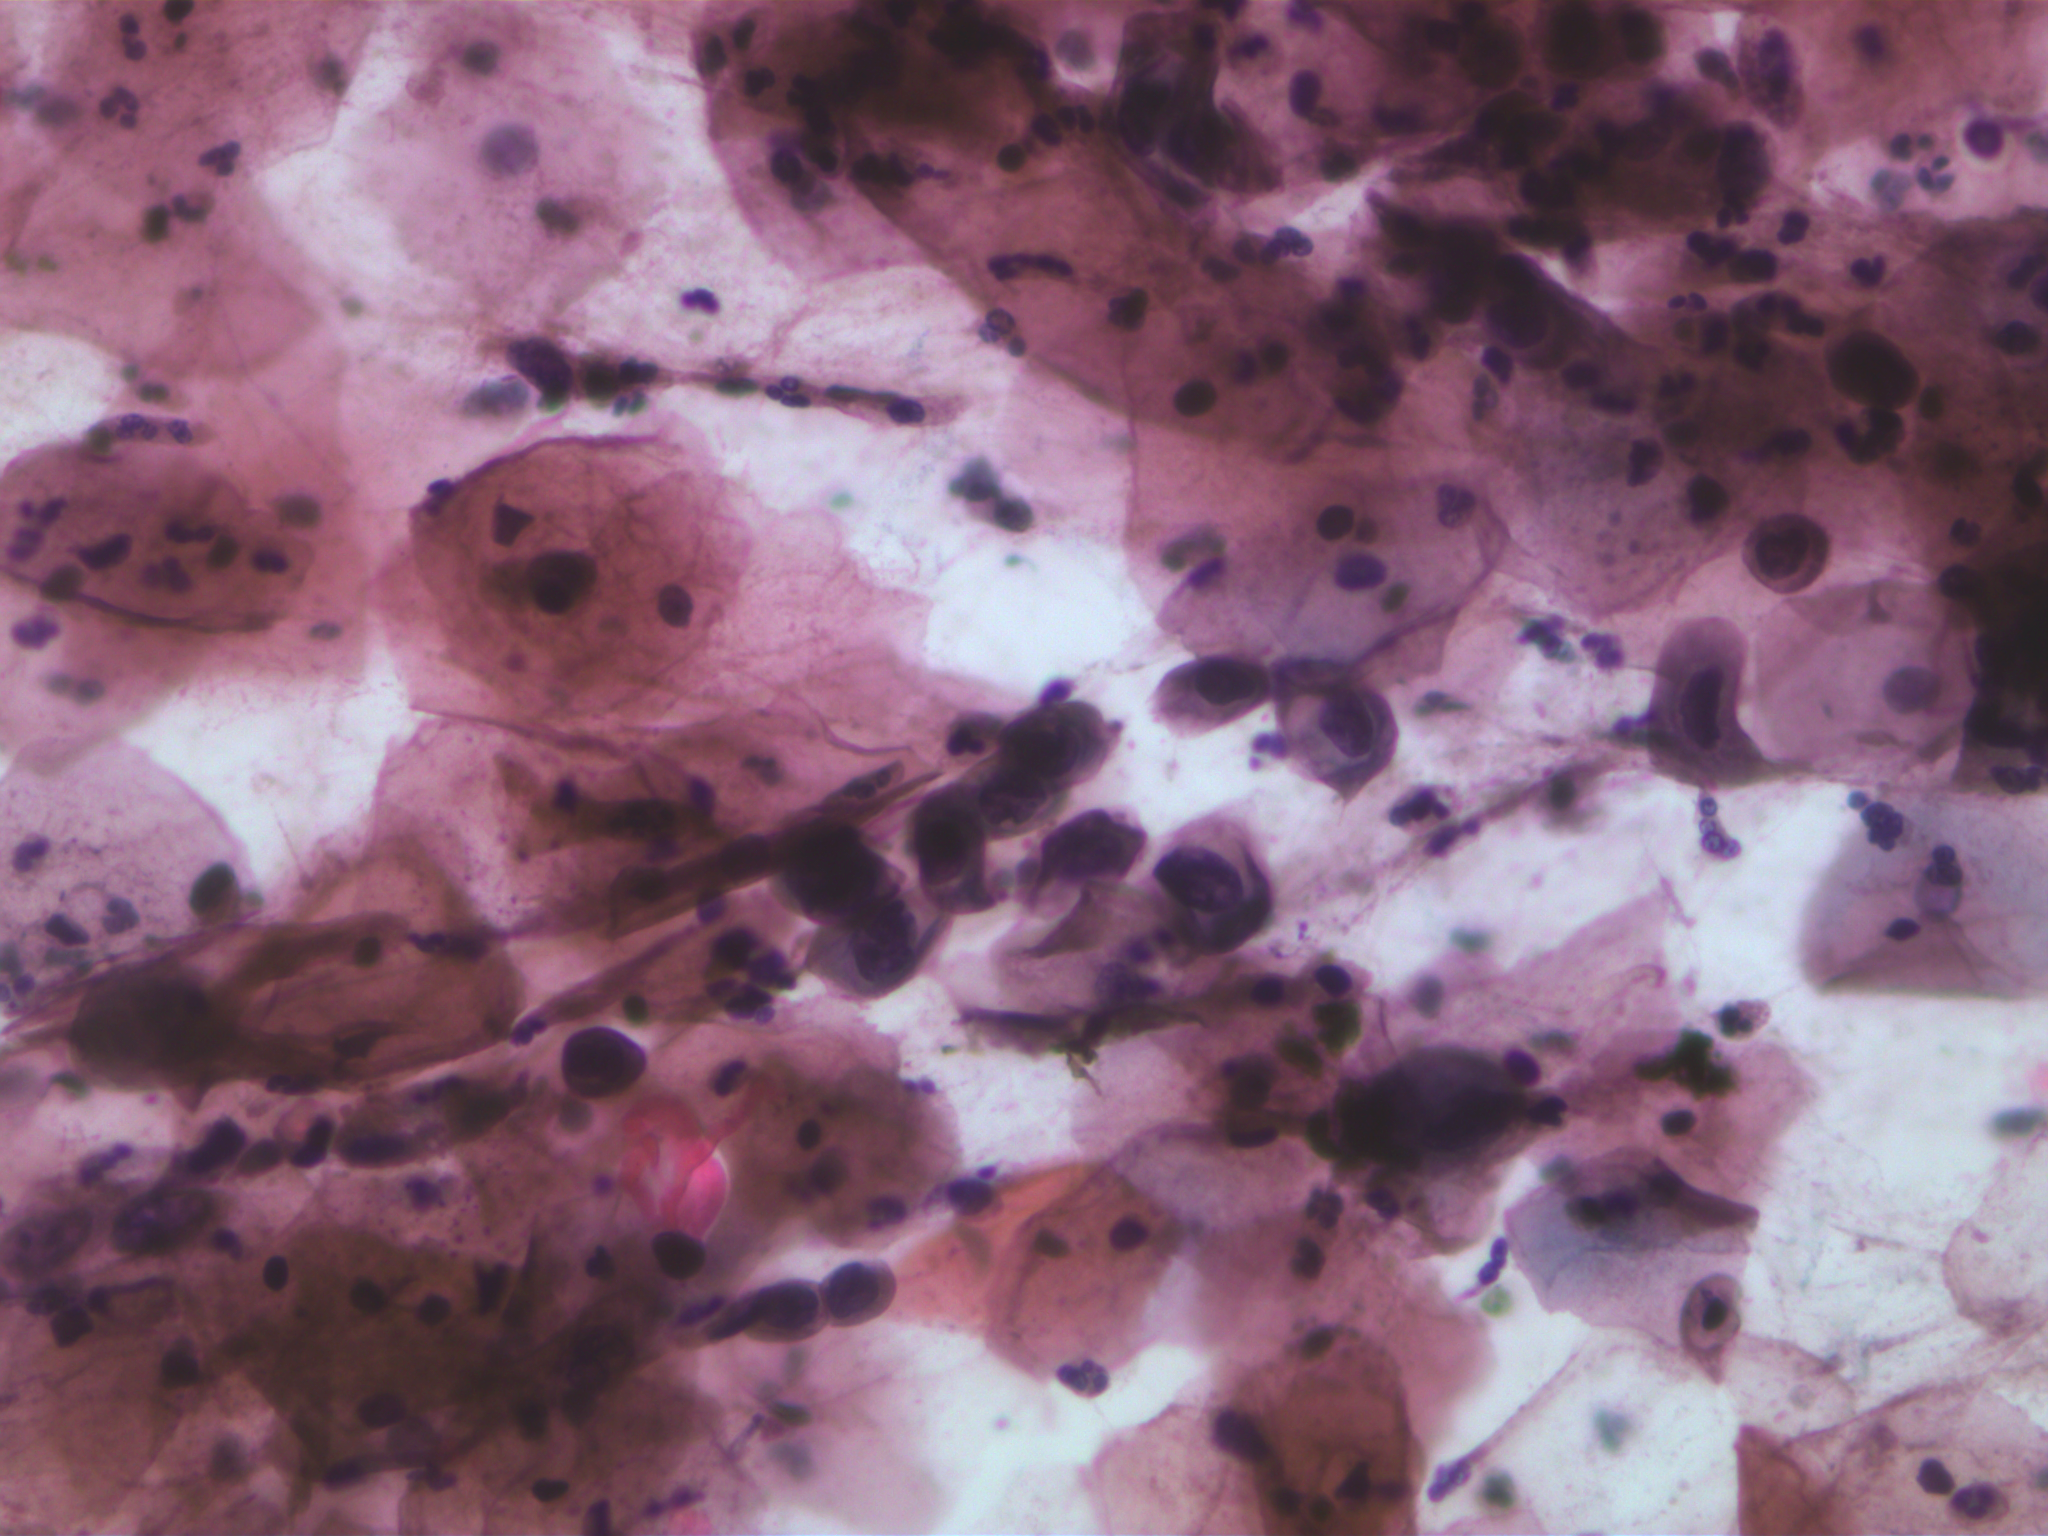
\includegraphics[width=0.30\textwidth]{cells/koilocytotic_110}} \quad
  \subcaptionbox{Metaplastic}{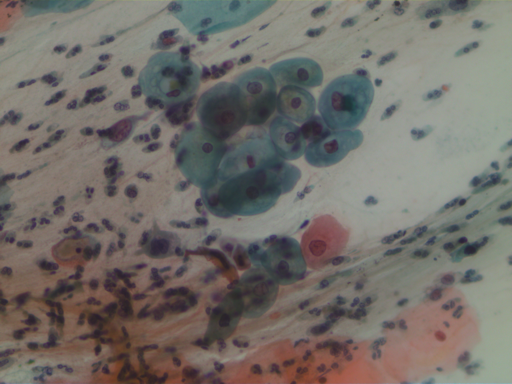
\includegraphics[width=0.30\textwidth]{cells/metaplastic_001}}%
  \hfill
  \subcaptionbox{Parabasal}{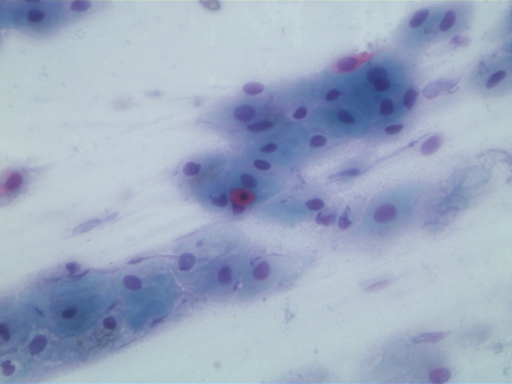
\includegraphics[width=0.30\textwidth]{cells/parabasal_020}} \quad
  \subcaptionbox{Superficial-Intermediate}{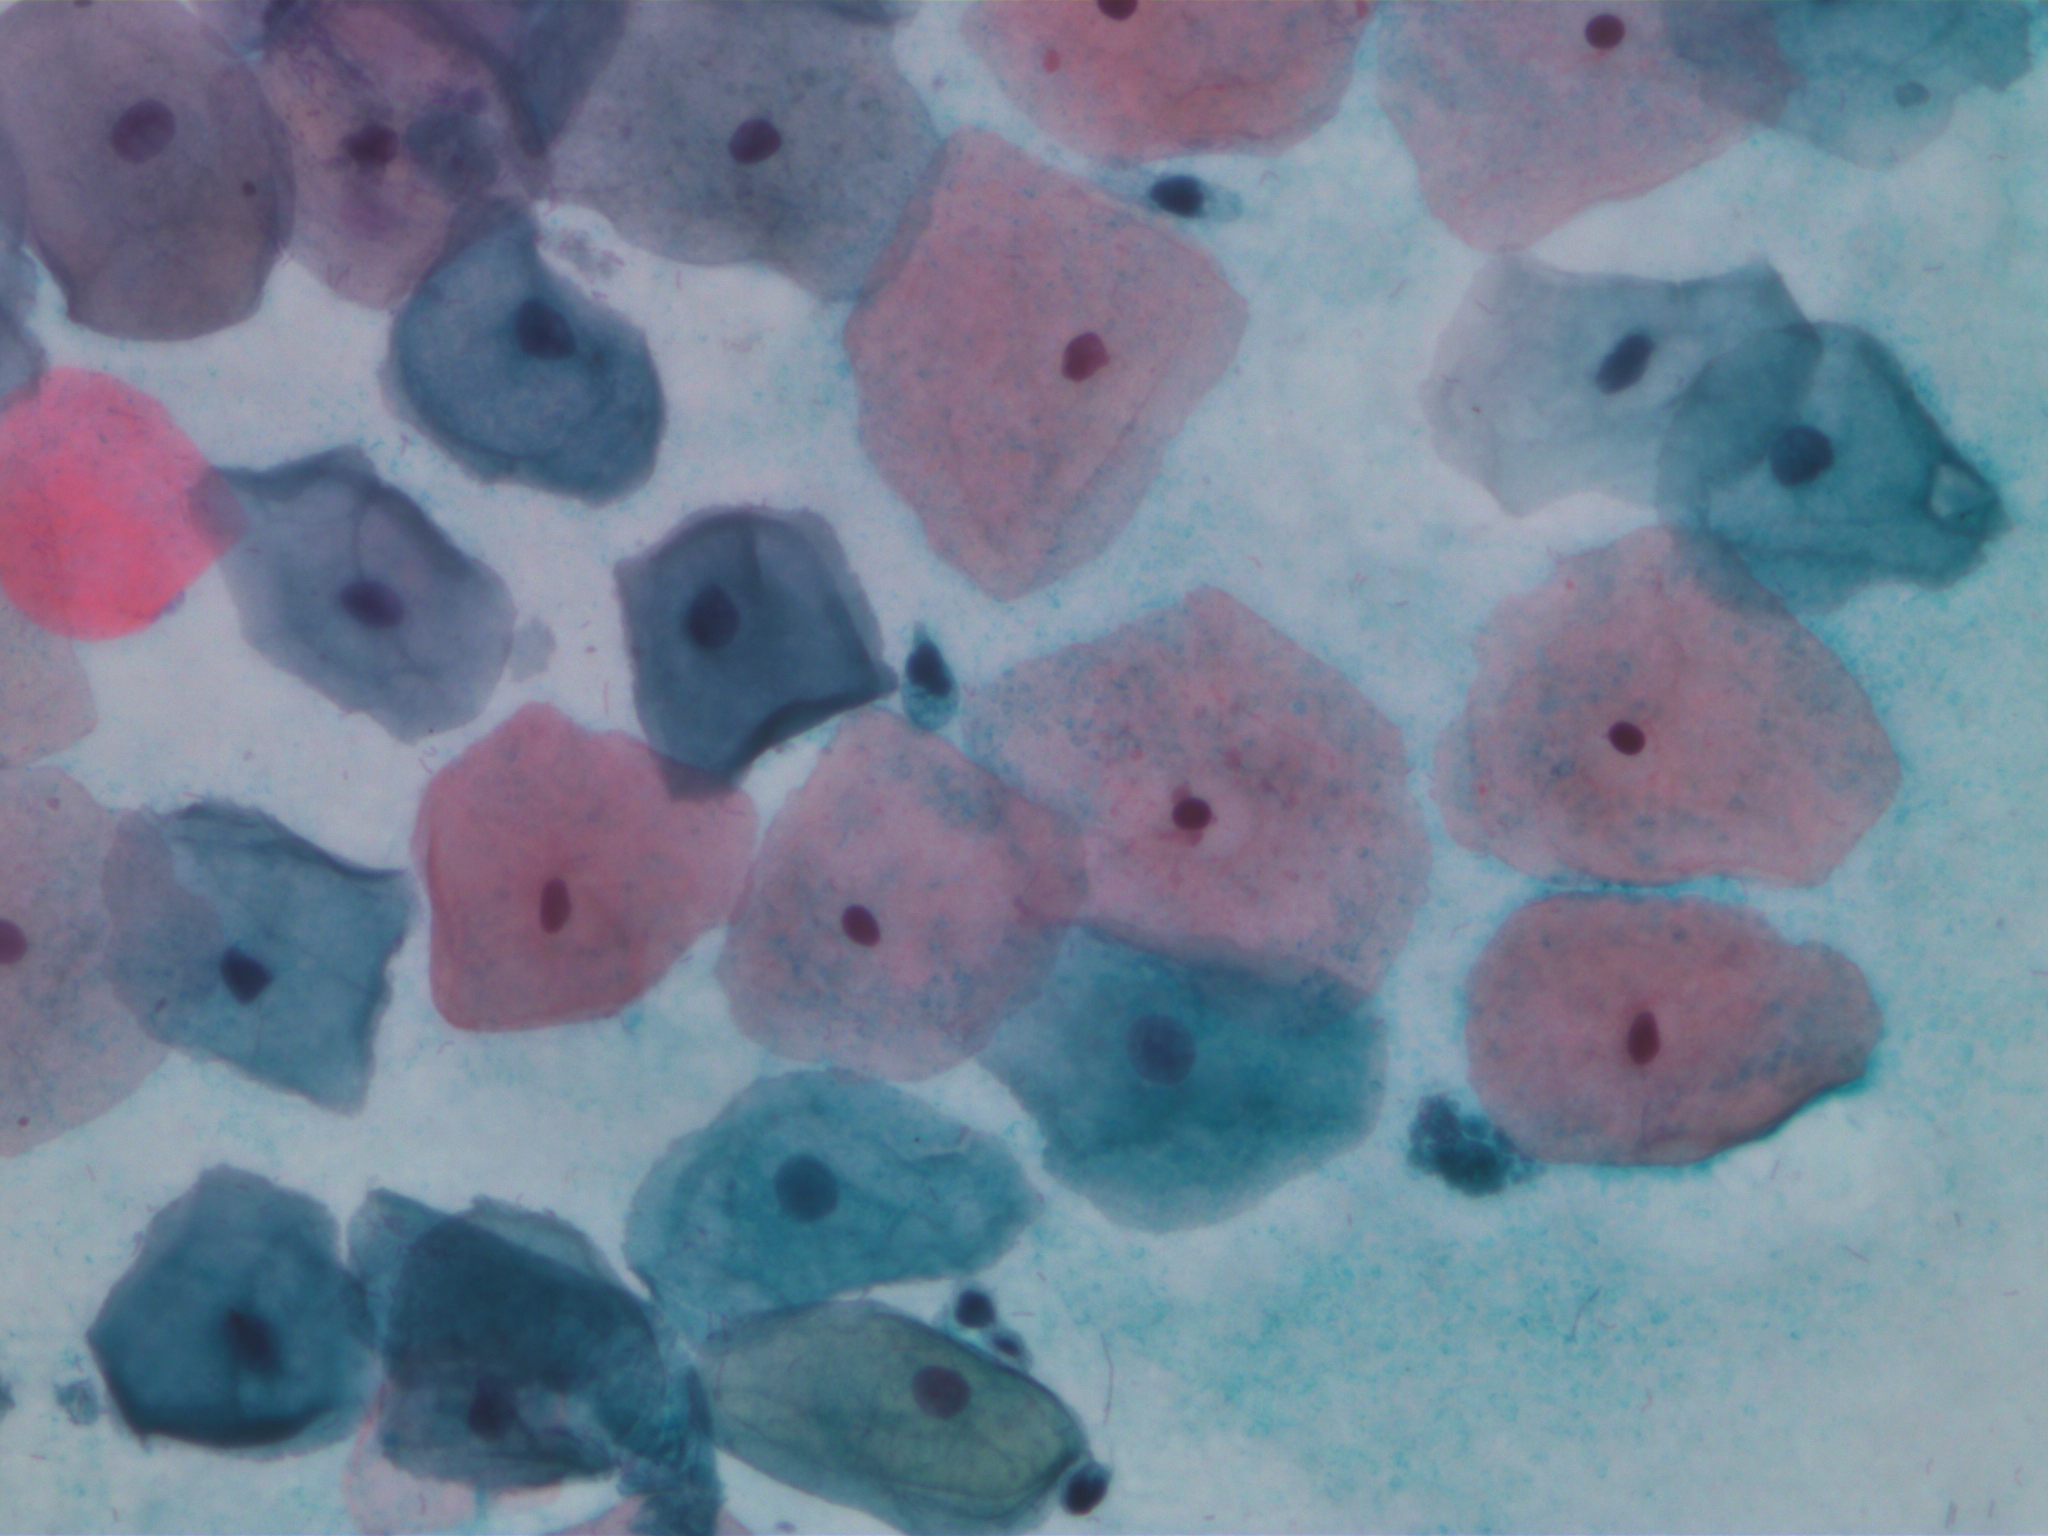
\includegraphics[width=0.30\textwidth]{cells/superficial_intermediate_007}} 
  \caption{Cell Types}
\end{figure}

\noindent \textbf{Superficial-Intermediate cells} constitute the majority of the cells found in a Pap test. Usually they are flat with round, oval or polygonal shape cytoplasm stains mostly eosinophilic or cyanophilic. They contain a central pycnotic nucleus. They have well defined, large polygonal cytoplasm and easily recognized nuclear limits (small pycnotic in the superficial and vesicular nuclei in intermediate cells). These type of cells show the characteristics morphological changes (koilocytic atypia) due to more severe lessions.
\\ \textbf{Parabasal cells} are immature squamous cells and they are the smallest epithelial cells seen on a typical vaginal smear. The cytoplasm is generally cyanophilic and they usually contain a large vesicular nucleus. It must be noted that parabasal cells have similar morphological characteristic with the cells identified as metaplastic cells and it is difficult to be distinguished from them.    
\\ \textbf{Koilocytotic cells} correspond most commonly in mature squamous cells (intermediate and superficial) and some times in metaplastic type koilocytotic cells. They appear most often cyanophilic, very lightly stained and they are characterized by a large perinuclear cavity. The periphery of the cytoplasm is very dense stained. The nuclei of koilocytes are usually enlarged, eccentrically located, hyperchromatic and exhibit irregularity of the nuclear membrane contour. 
\\ \textbf{Dysketarotic cells} are squamous cells which undergone premature abnormal keratinization within individual cells or more often in three-dimensional clusters. They exhibit a brilliant orangeophilic cytoplasm. They are characterized by the presence of vesicular nuclei, identical to the nuclei of koilcytotic cells. In many cases there are binucleated and/or multinucleated cells.
\\ \textbf{Metaplastic Cells} are small or large parabasal-type cells with prominent cellular borders, often exhibiting eccentric nuclei and sometimes containing a large intracellular vacuole. The staining in the center portion is usually light brown and it often differs from that in the marginal portion. Also, there is essentially a darker-stained cytoplasm and they exhibit great uniformity of size and shape compared to the parabasal cells, as their characteristic is the well defined, almost round shape of cytoplasm.\cite{sipakmed}

\section{Herlev}
The Herlev dataset is comprised of 917 isolated single cell images. These are distributed unequally between seven classes of cells.  Superficial squamous epithelia, intermediate squamous epithelia, columnar epithelial, mild squamous non-keratinizing dysplasia, moderate squamous non-keratinizing dysplasia, severe squamous non-keratinizing dysplasia and squamous cell carcinoma in situ intermediate.\cite{herlev}

\begin{figure}[H]
  \centering
  \subcaptionbox*{Light Dysplastic}{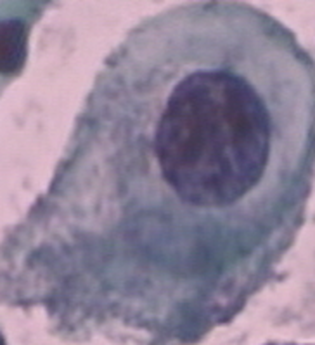
\includegraphics[width=.21\textwidth]{cells/herlev/light_dysplastic}} \quad
  \subcaptionbox*{Moderate Dysplastic}{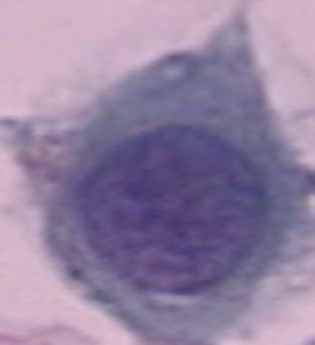
\includegraphics[width=.21\textwidth]{cells/herlev/moderate_dysplastic}} \quad
  \subcaptionbox*{Severe Dysplastic}{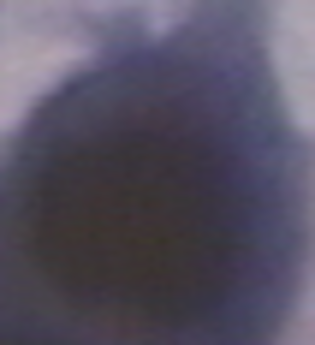
\includegraphics[width=.21\textwidth]{cells/herlev/severe_dyplastic}} \quad
  \subcaptionbox*{Carcinoma in Situ}{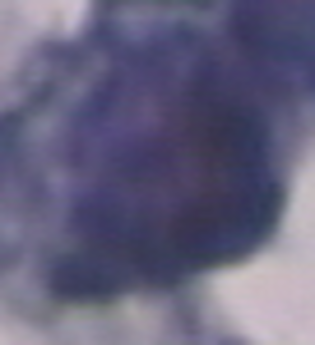
\includegraphics[width=.21\textwidth]{cells/herlev/carcinoma_in_situ}}
  \caption{Abnormal Cells}
\end{figure}
\begin{figure}[H]
  \centering
  \subcaptionbox*{Intermediate}{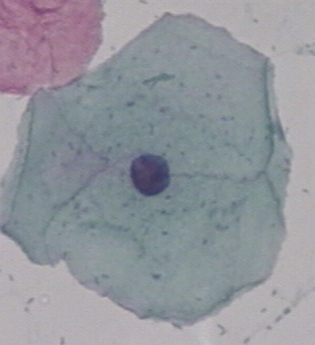
\includegraphics[width=.21\textwidth]{cells/herlev/normal_intermediate}} \quad
  \subcaptionbox*{Superficiel}{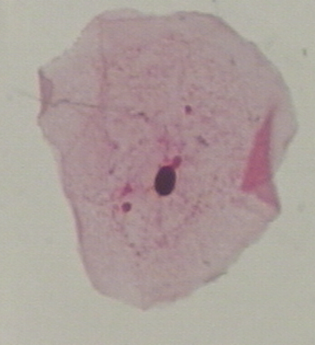
\includegraphics[width=.21\textwidth]{cells/herlev/normal_superficiel}} \quad
  \subcaptionbox*{Columnar}{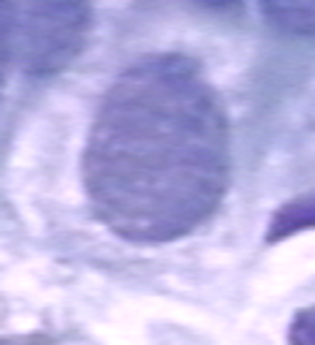
\includegraphics[width=.21\textwidth]{cells/herlev/normal_columnar}}
  \caption{Normal Cells}
\end{figure}


\chapter{Background}

Current automatic screening scystems that incorperate pap smear have a very similar workflow: cell segmentation, cytoplasm and nuclei segmentation, feature extraction, and cell classification.

Whole slide classification (no segmentation) \cite{kiran}

\chapter{Synthetic Data Generation}

\begin{itemize}
  \item rotations
  \item flip horizontal and vertical
  \item random crop and zoom
\end{itemize}


\chapter{Segmentation Model}
\chapter{Experiments and Reuslts}

\chapter{Future Work}

\chapter{Tools and skills learned}

\chapter*{Project Requirments}

\section{Project Initiation}
The student finds a mentor who agrees to work with him/her on a project not later than the end of his/her 3rd semester in the program. The project may be initiated by the student or the mentor. 
 

\section{Project Development and Completion}

When the student is ready to complete the project, the student signs up for CS 698R (add code should be obtained from the Graduate Academic Advisor). The student will be expected to put 125-150 hours of work into the project during that semester. CS 698R is a pass/fail class. It is expected that students will only take this class once. The proposal form must be completed, signed and turned into the Graduate Academic Advisor by the first day of classes in the semester/term you intend to take the course.

The student prepares a short proposal and submits it to the graduate coordinator by the end of the first week of the semester.  The proposal focuses on specific activities and clearly-defined deliverables, approved by the mentor and then by the graduate coordinator.  The proposal should include a checklist of deliverables that will be demonstrated in the final presentation.
The mentor and student meet at least weekly throughout the project so that the student has a meaningful mentoring experience. The mentor must approve all revisions to the project deliverables checklist.
The student tracks hours worked on the project and keeps a week-by-week log of hours spent working on the project, split into categories such as design, coding, writing, etc. This 1) allows the mentor to make sure that expectations are met, 2) helps curb project creep, and 3) is common practice in industry (particularly if working for a company that handles multiple consulting/contracts/projects, where it is important to track to the fraction of an hour how long is spent on each).
By the middle of the semester (by the end of the 9th week), the student produces a draft report, also focused on deliverables, a copy of which must be submitted to the Graduate Coordinator. An email will be sent to all faculty mentors and MS Project students by the end of 7th week of the semester as a reminder of this requirement. The student and mentor discuss the draft report, review the time log, go over the write-up, and make scope adjustments if needed. This contributes to the student having a meaningful and culminating writing experience.  Additional reviewing iterations are recommended, but optional.
The student prepares a final written scientific project report, including at least an executive summary, an introduction, a project description, a validation section, and a conclusion.
At the end of the semester, project presentations are held within a 3-hour block during finals week. Two members of the Graduate Committee, together with the mentor for each project, make up the student's committee. The Committee sits at a desk with all the project reports in a binder in order of student presentation. The students present for 15 minutes after which there are 5 minutes for questions and comments. The Committee reviews the time log, and checks off deliverables as the student presents. If all deliverables are satisfactory, the student passes. If not, the Committee may discuss and advise as to whether the student passes or fails.
Project Report
The MS project report document should be submitted to the committee at the end of the semester in which the student takes CS 698R. The document must be about 15 double-spaced pages. The project report should provide necessary background and then argue that a significant piece of work was needed. The contributions should reflect the importance of the work. A summary of the project's time log must also be included. 

\section{Project Report Presentation }

Oral Presentation Audience: CS faculty members who may not be acquainted with the topic.

A 12-15 minute oral presentation of the project must be carefully organized and given to the members of the MS committee and the invited public. During the project report presentation, the student must answer committee member's questions on such areas as method, significance, organization, and literature search. After the presentation, the student and public leave the room while the committee comes to a decision on project report. 
 

Examination Results:

At this point the examining committee decides on a result. The possible results are:

Pass

Pass with qualifications - Revision to project is an example of why this would be selected.

Fail - Fail the oral exam and be terminated from the graduate program.

The final CS 698R grade will be determined by the Advisor

\bibliographystyle{plainnat}
\bibliography{bib}
\end{document}
